\section{Practical measurement considerations}
Some practical measurement considerations can have a considerable effect on the localization results. For instance, the delay table that is computed for the SRP-MAP has a maximum magnitude, \textit{d}. This is because the microphone array can measure signal delays only within a finite value. Thus, \textit{d} is the number of samples that can fit within two microphones of the array. Obviously, \textit{d} depends on the array aperture and also the sample rate of recording. Higher \textit{d} values are preferable as that directly translates to a higher achievable resolution on the SRP-MAP (\ref{app:angRes}).
\subsubsection{Effect of array aperture and sample rate}
As discussed above and shown in Fig. \ref{fig:res_diff}, reducing the aperture size or sample rate also reduces the angular resolution of localization, which causes a direct degradation in SRP-PHAT performance. Fig. \ref{fig:4mic1srcAper} depicts the effect of reducing sample rate or aperture size on the SRP-PHAT localization results. Any reduction in the array aperture of the sample rate causes the localization circles to become annular. This is because more $\theta$s and $\phi$s correspond to the same integral delay. These issues can be somewhat alleviated if the algorithm considered fractional delays and interpolation. However, even with interpolation, some data between the integral delays is always lost. For the outdoor localization, a sample rate of 131072Hz is used, which results in an angular resolution of 
\begin{figure}[H]
    \centering
    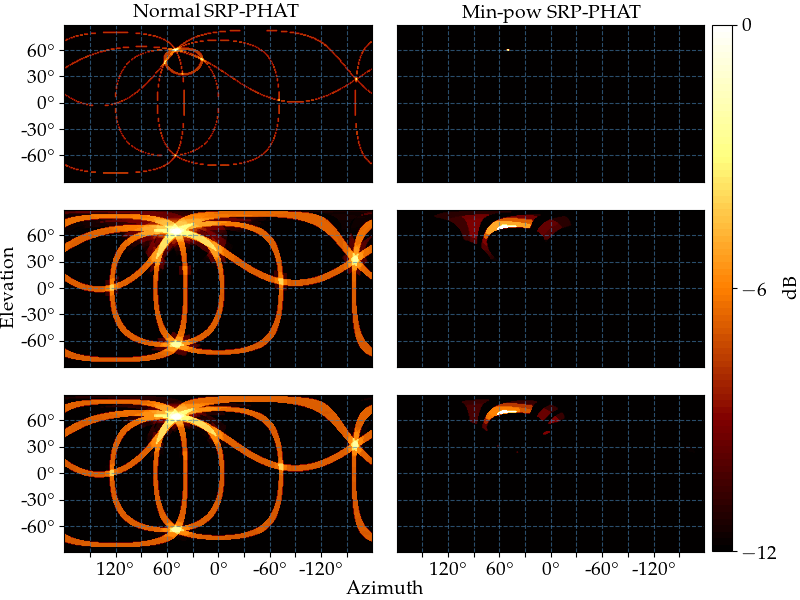
\includegraphics[width=\textwidth]{Figures/aperSampSim.png}
    \caption{Figures depict from top-to-bottom SRP-PHAT localization results with tetrahedral microphone array aperture size of 1m@48kHz, 10cm@48khz and 1m@4.8kHz.}
    \label{fig:4mic1srcAper}
\end{figure}
\subsubsection{Effect of audio recording length}
\begin{figure}[H]
    \centering
    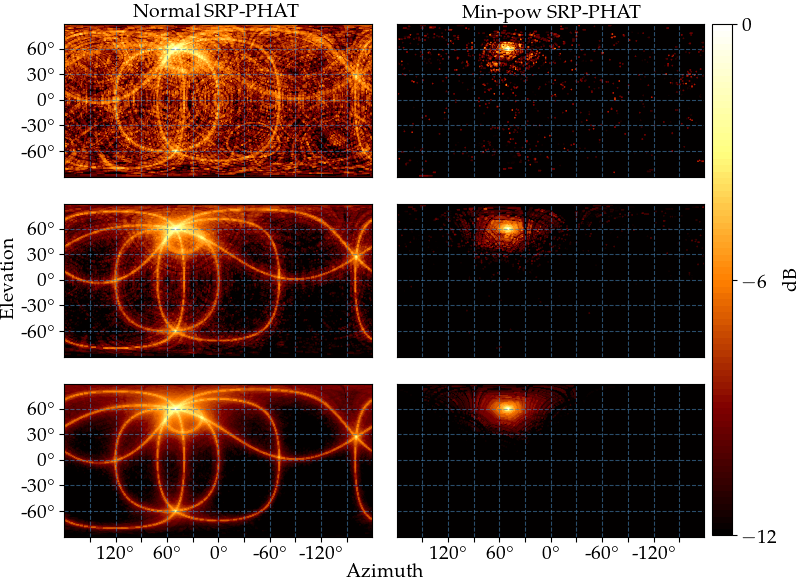
\includegraphics[width=\textwidth]{Figures/audioLenSim.png}
    \caption{Figures depict from top-to-bottom SRP-PHAT localization results with tetrahedral microphone array with recording length of 1sec  (top), 10sec (middle) and 100sec (bottom)}
    \label{fig:micErrTilt}
\end{figure}
%\subsubsection{Effect of adding more microphones}
%It is of interest to test the scalability of the algorithm by adding more microphones. Theoretically, adding microphones should add independent pairs and thus lower the noise floor (normalized) to improve results in a low SNR scenario. 
%\begin{figure}[H]
%\begin{subfigure}[b]{0.96\textwidth}
%    \centering
%    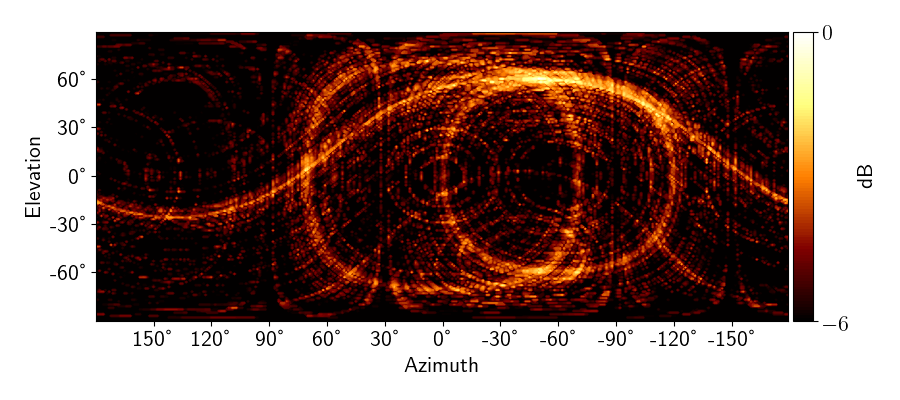
\includegraphics[width=0.8\textwidth]{Figures/Ind4mic1srcResNeg10LowDyn.png}
%\end{subfigure}
%\vskip \baselineskip
%\begin{subfigure}[b]{0.96\textwidth}
%    \centering
%    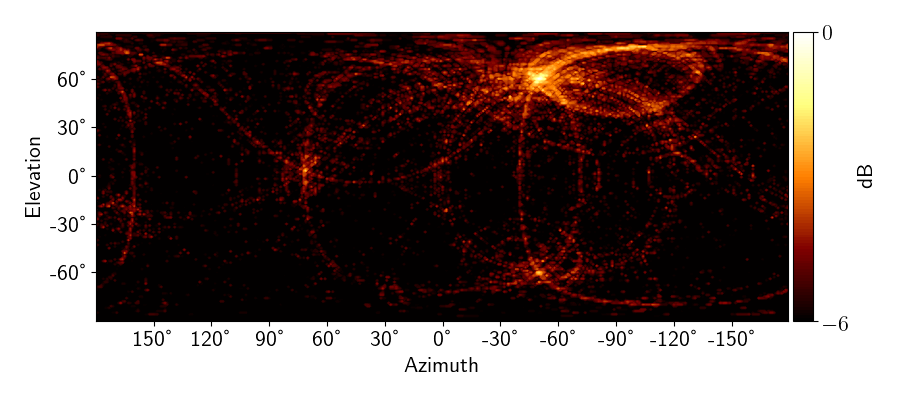
\includegraphics[width=0.8\textwidth]{Figures/Dep4mic1srcResNeg10LowDyn.png}
%\end{subfigure}
%\caption{Figures depict from SRP-PHAT localization results with SNR = -10dB, for independent microphone pairs (top), and for all  microphone pairs (bottom)}
%\label{fig:4mic1srcRedun}
%\end{figure}
\
\subsubsection{Effect of error in mic position}
The microphones in the array could have an error in position, due to structural errors (structural fatigue and sag, thermal expansion/ contraction or just human error). This could lead to an error in localization. Fig. \ref{fig:micErrPos} illustrates this effect. 
\begin{figure}[H]
    \centering
    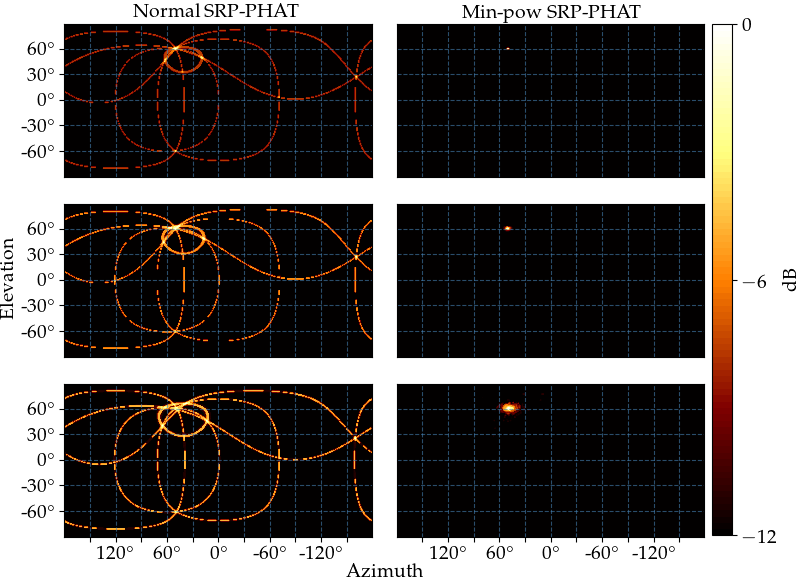
\includegraphics[width=\textwidth]{Figures/micErrPosSim.png}
    \caption{Figures depict from top-to-bottom SRP-PHAT localization results with tetrahedral microphone array with no mic error in placement (top), a 1cm placement error in 1 mic (middle), a 2cm placement error in all mics (bottom)}
    \label{fig:micErrPos}
\end{figure}

\subsubsection{Effect of error in array tilt}
\begin{figure}[H]
    \centering
    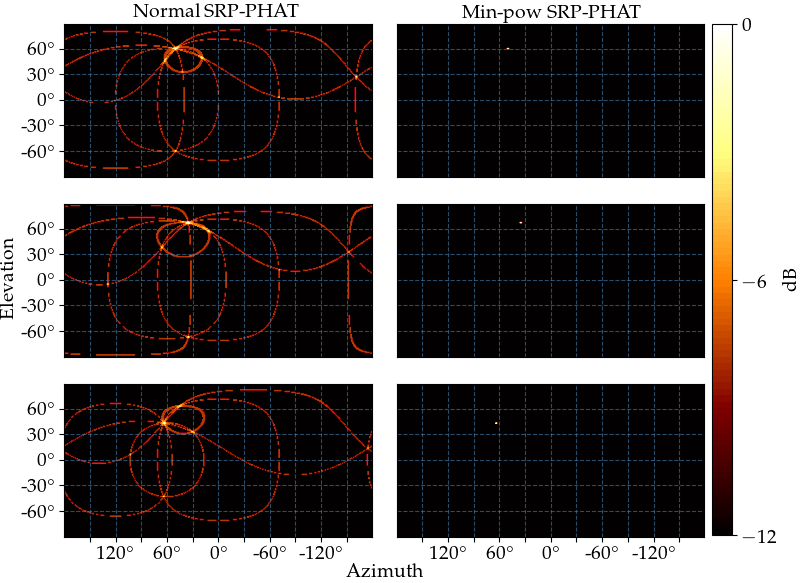
\includegraphics[width=\textwidth]{Figures/micErrTiltSim.png}
    \caption{Figures depict from top-to-bottom SRP-PHAT localization results with tetrahedral microphone array with no mic tilt error (top), a +10$\degree$ tilt  error (middle) along the x-axis and a -20$\degree$ tilt error along the x-axis (bottom)}
    \label{fig:micErrTilt}
\end{figure}


